
\section{Introduction}

A desire for robotic solutions, particularly in the Small and Medium scale
Enterprises (SMEs) is becoming increasingly prominent. Automation and robotics
promise to deliver reduction on production costs and increase in productivity.
However, traditional automation implies an investment prohibitive for SMEs,
whose activities mainly involve small batches of production and high variety of
products, for example, due to a seasonal nature of their operations.
Concretely, tasks such as assembly, machine filling or packaging, can be
automated with a robot in the workcell. However economic feasibility requires to
reduce the robotization costs. The Factory-in-a-day project \cite{fiad} tries to reduce the
robotization cost by reducing the system integration cost and installation time.
The key idea is that the robot solution is flexible so that it can be quickly
re-installed and configured to another temporary product line.


To achieve this flexibility and maintain acceptable levels of productivity, in
the Factory-in-a-day approach we propose to automate the easy 80\% of the tasks
and leave the hard 20\% for human co-workers. Robot manipulators provide power,
repeatability and extended work-space while the human operators provide
flexibility and problem solving capacity. In addition, fenceless collaborative
robots save space and installation cost. However, this approach requires a very
high level of safety and agility; the robots should be aware of any obstacle,
including dynamic obstacles such as its humans co-workers, and be able to move
to avoid contact. Whereas current co-bots guarantee safe contacts, they degrade
the performance of the work cell because of stopping the production. This is one
of the breakthrough innovations of the Factory-in-a-day project, which is the
focus of this paper: robot arms that are aware of all (dynamic) obstacles in
their environment, and that respond by moving around these obstacles while
still continuing their work. 




Since a 6-axis robot was designed at Stanford allowing a systematic way to design a robot and compute Inverse Kinematic solution analytically in the seventies, robots have been widely used for a variety of applications from punching cards and palletizing food items to assembly and welding in big automobile manfucaturing lines and intelligent stock handling in warehouses \cite{scheinman1969design}. Safety and reliability became a significantly potential area of research since then \cite{dhillon2012robot}. These robots are usually installed in closed chambers, fixed on the ground and absolute care is taken not to make it operational when the door is open or when the co-worker is around the robot's workspace \cite{safetyreqs}.
The safety guidelines are obviously strict as it is crucial to avoid humans in danger. But things are changing quite rapidly and we have an increased focus on human-robot colloboration with enhanced safety in the last decade \cite{Bicchi2008,dhillon2012robot} driven by creative industrial demands and high interest in flexible mobile manipulators. The safety is evaluated based on various factors influencing the human-robot collision impact such as the proximity distance, relative velocity, robot inertia and so on \cite{Kulic2006}. One of the main requirement is the robot's capability to perceive the environment and react to it and this paper focuses on the same. 

%    \begin{figure}[thpb]
%       \centering
%       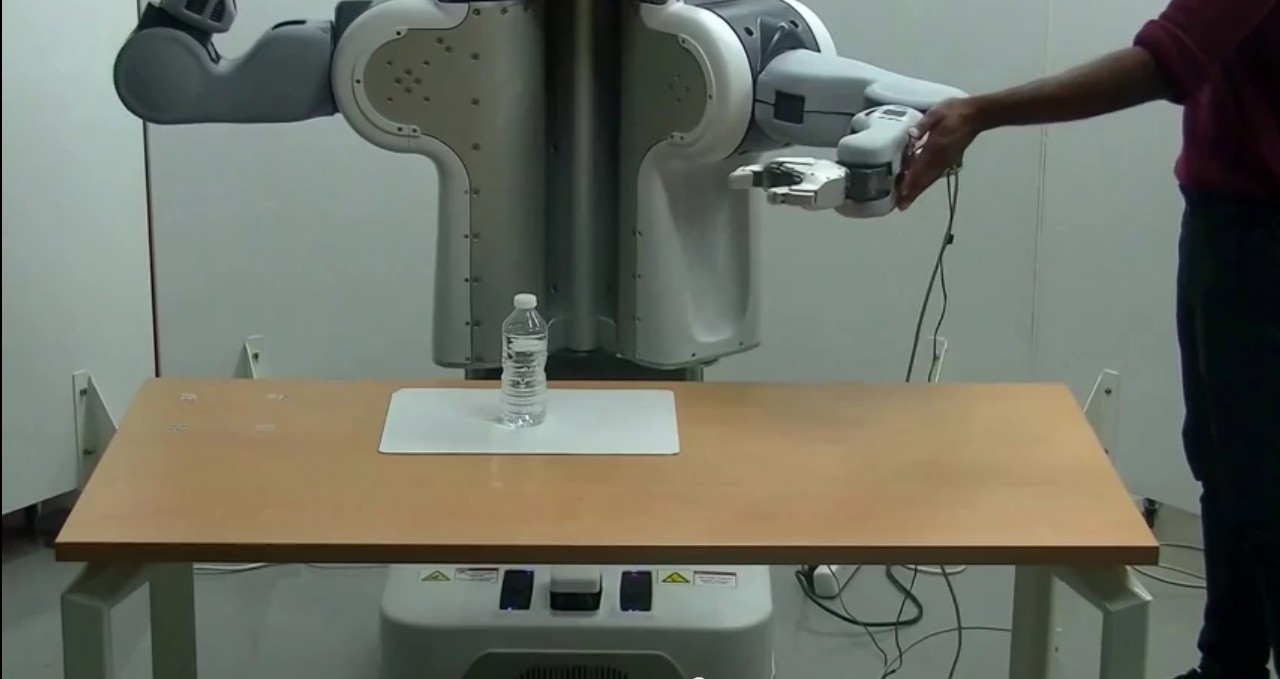
\includegraphics[scale=0.2]{doa/images/skin.eps}
%       \caption{A mobile manipulator executing a trajectory to reach a pre-grasp pose while the forearm is approached by a person with his hand. A skin sensor mounted on the forearm is used to sense any obstacle in the proximity. }
%       \label{figurelabel}
%    \end{figure}

Collision avoidance is an important requirement in terms of safety and has been a well researched topic. Various approaches have been used to handle different scenarios. In the earlier times, the approaches model the obstacles as static entities and treat them as a planning problem to avoid collisions \cite{van2011reciprocal}. Replanning is performed based on instantaneous observations if the obstacles are moving. These planning based approaches limit the low level control to simple operations with controller frequencies several times smaller than robot-environment interation time. Constrained based approaches focus on enhancing low level control to perform complex operations
by taking sensor data directly to be reactive enough with the environment \cite{khatib1986real}. Collision avoidance can be modeled as inequality constraints. There are a variety of possible inequalities both in robot and environment in robot application scenarios. Some examples are joint limits, singularity avoidance, and object tracking in visual servoing. Equalities usually model the main goals of a scenario or hard constraints. Constraints based robot programming were used extensively to solve these constraints in the local control but were specific to robot and the scenario involved. 
   
Redundant systems are increasingly popular due to their increased flexibility of arm and a mobile base to handle inequalities constraints. The control of redundant robots is difficult as it is not always easy to compute inverse kinematic and dynamic solutions in closed form. The control techniques to solve redundancy mostly uses task function based approach to minimize the error in task space\cite{Samson1991}. They are jacobian based techniques inverting the differential mapping that maps the control space and the error space to compute optimal controller outputs. A systematic framework for redundant system control proposed by Siciliano allowed to execute multiple tasks simultaneously with priorities \cite{siciliano1991general}. These framework can only solve equality tasks and various strategies focuses on transforming inequality constraints to equalities\cite{Nelson95strategiesfor}\cite{chan1995weighted}\cite{mansard2009directional}\cite{raunhardt2007progressive}. These strategies are not generic enough and has priority inversion problems making them unreliable for practical use.

A cascade approach was alternatively used to represent the inequalities and equalities systematically as a hierarchical least quare program\cite{kanoun2011kinematic} but it was not fast enough to be used in real time to handle inequalities. Recently proposed hierarchical quadratic program(HQP) solver uses complete orthogonal decomposition (COD) instead of singular value decomposition (SVD) and an improved search algorithm which makes it more efficient than available solvers\cite{escande2014hierarchical}. Though constraint based approaches are quite an efficient way to handle collisions and a flexibile way to model them, the are merely locally optimal controllers and does not provide a systematic way to escape local minima. This necessitates the support of global path planners to find the optimal
path for realizing a robot task. Combining global path planning and a reliable reactive control is an essential need for deploying robots from simple to complex scenarios and this addressed in this paper. 

This work is a direct application of the HQP solver and a first attempt to combine path planning and reactive control in a jacobian based solver framework eliminating a cumbersome architecture handling the information flow between control and planning components. Stack of Tasks, a controller framework that implements the latest HQP solver is used in this work to apply the proposed methodology. The proposed methodology is tested on PR2, a mobile manipulation platform with a skin sensor mounted on the forearm of the robot to demonstrate the collision avoidance while executing a planned trajectory without compromising the final goal of the scenario. 


The paper is organised as follows. Section \ref{sec:application} describes the solution for dynamic obstacle avoidance and Section \ref{sec:skin} discusses the proximity-sensing robot skin. In Section \ref{sec:sot} the robot motion control architecture to incorporate the collision information as safety
constraints to dynamically adapt the trajectory is presented. Section \ref{sec:prelim_results}
presents the preliminary results obtained in two different robot setups. Finally, in Section \ref{sec:conclusions} we present our concluding remarks and a discussion of the current work in progress.
